\chapter{ Testes }

Neste capítulo são apresentados os testes realizados no sistema
proposto com a arquitetura de rede neural definida no capítulo
anterior. Todos os treinamentos foram realizados na infraestrutura
citada no capítulo de proposta do trabalho. Os resultados foram
satisfatórios para o conexto do trabalho. Para produzir os gráficos
foi utilizada um ferramenta chamada {\bf \emph{TensorBoard}}, que vem
junto com a instalação do \textit{TensorFlow}.

\section{Treinamento com 200 mil iterações}

Inicialmente realizamos um treinamento com 200 mil iterações, portanto
3.125 passos com uma carga de 64 imagens. A fase de treinamento
completa levou {\bf 1 hora 23 minutos e 54 segundos} para
completar. Deve-se salientar que para o primeiro treinamento há uma
espera maior devido ao \textit{caching} dos dados. Isso é feito pelo
sistema operacional para otimizar a memória da GPU e do sistema em
geral quando os dados são carregados para a memória volátil. 

Como é possível observar nos gráficos o valor da perda para este
treinamento oscila entre 17,02 e 17,93 até o passo número 2.050
(iteração 131.200) onde a perda começa a decair. O mesmo acontece com
a acurácia, ficando em torno de 5\% até o passo 2.050 quando começa a
subir. Ao final do treinamento foi alcançada uma acurácia de {\bf
  80,94\%} no conjunto de treinamento, {\bf 79,6\%} no conjunto de
teste e uma perda de {\bf 2,87} para o conjunto de treinamento, {\bf
  2,91} para o conjunto de teste.

\begin{figure}[H]
\centering
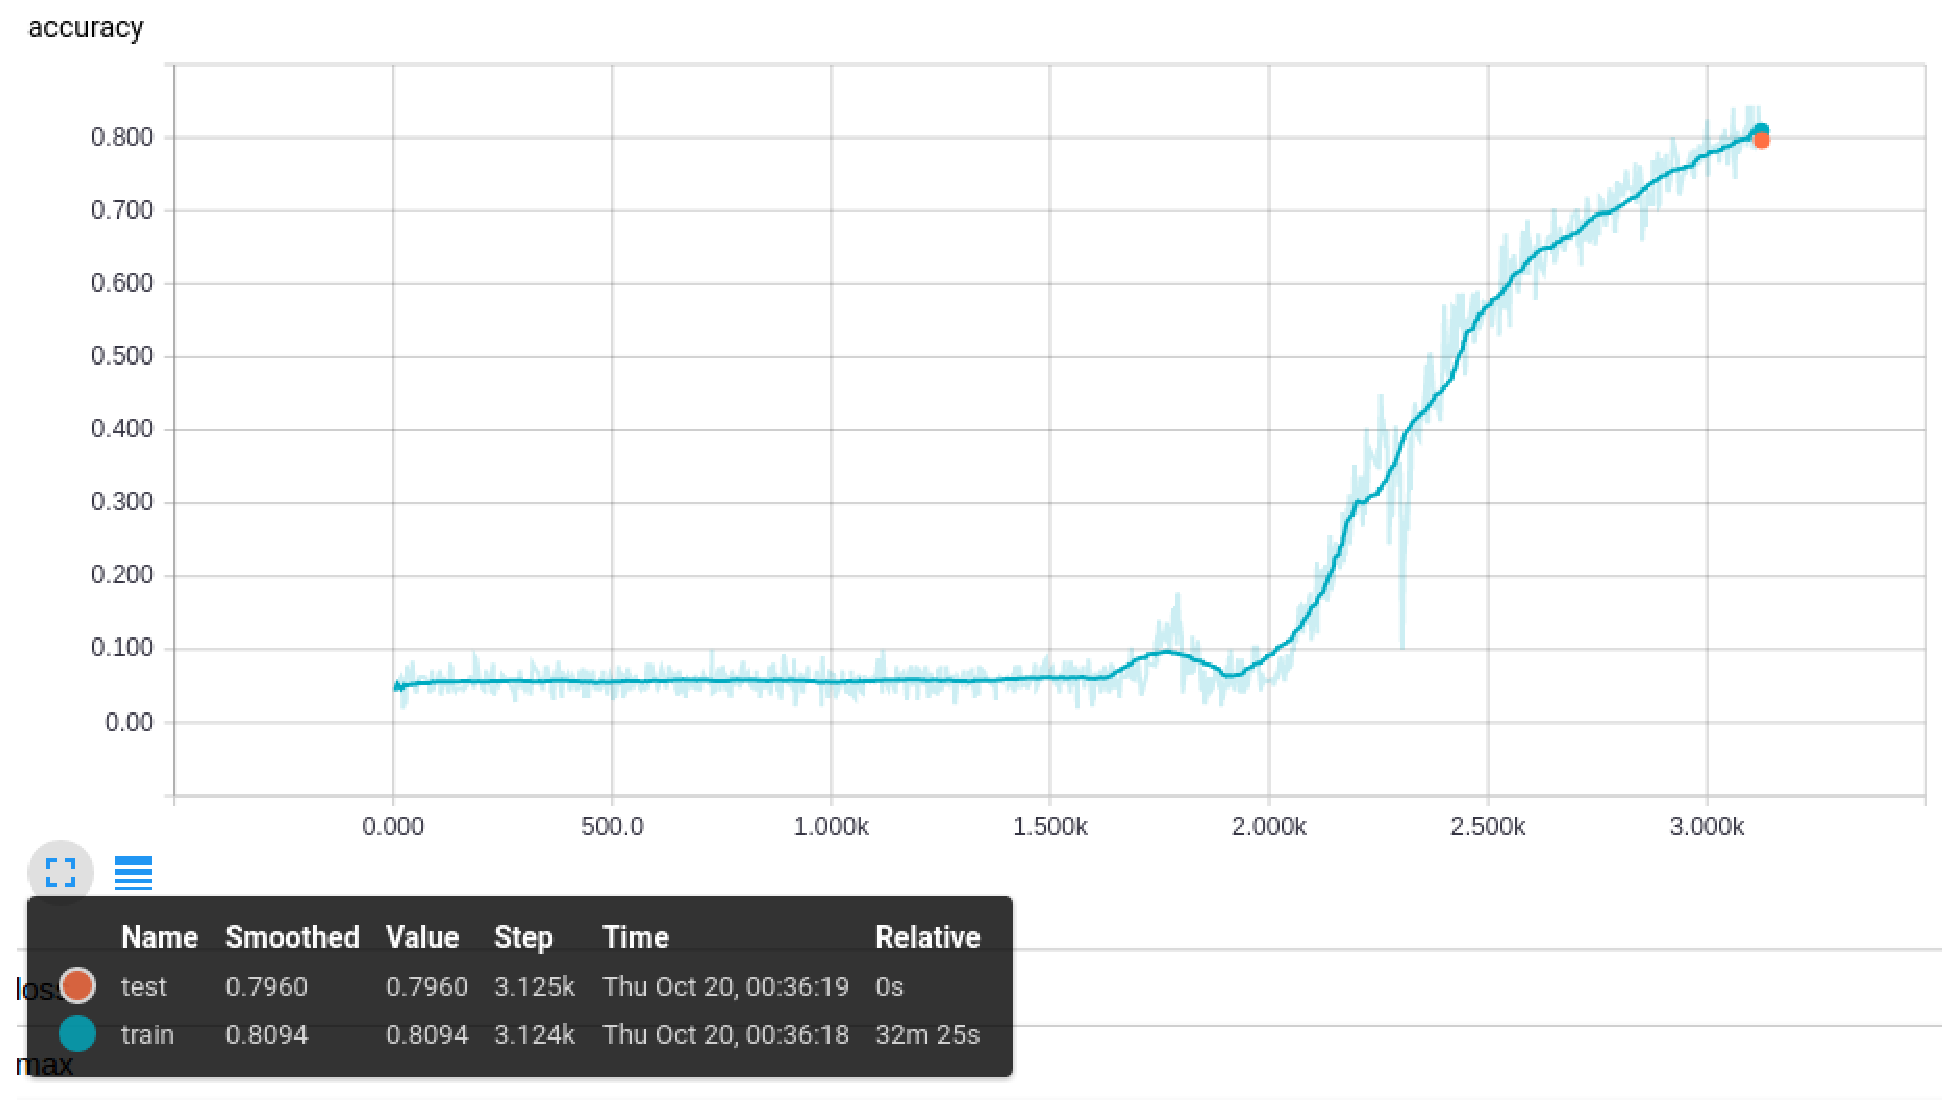
\includegraphics[scale=0.4]{imagens/accuracy_200k}
\caption{Gráfico da acurácia em relação ao número de passos para o
  treinamento da rede com 200 mil iterações.}
\label{fig:accuracy_200k}
\end{figure}

\begin{figure}[H]
\centering
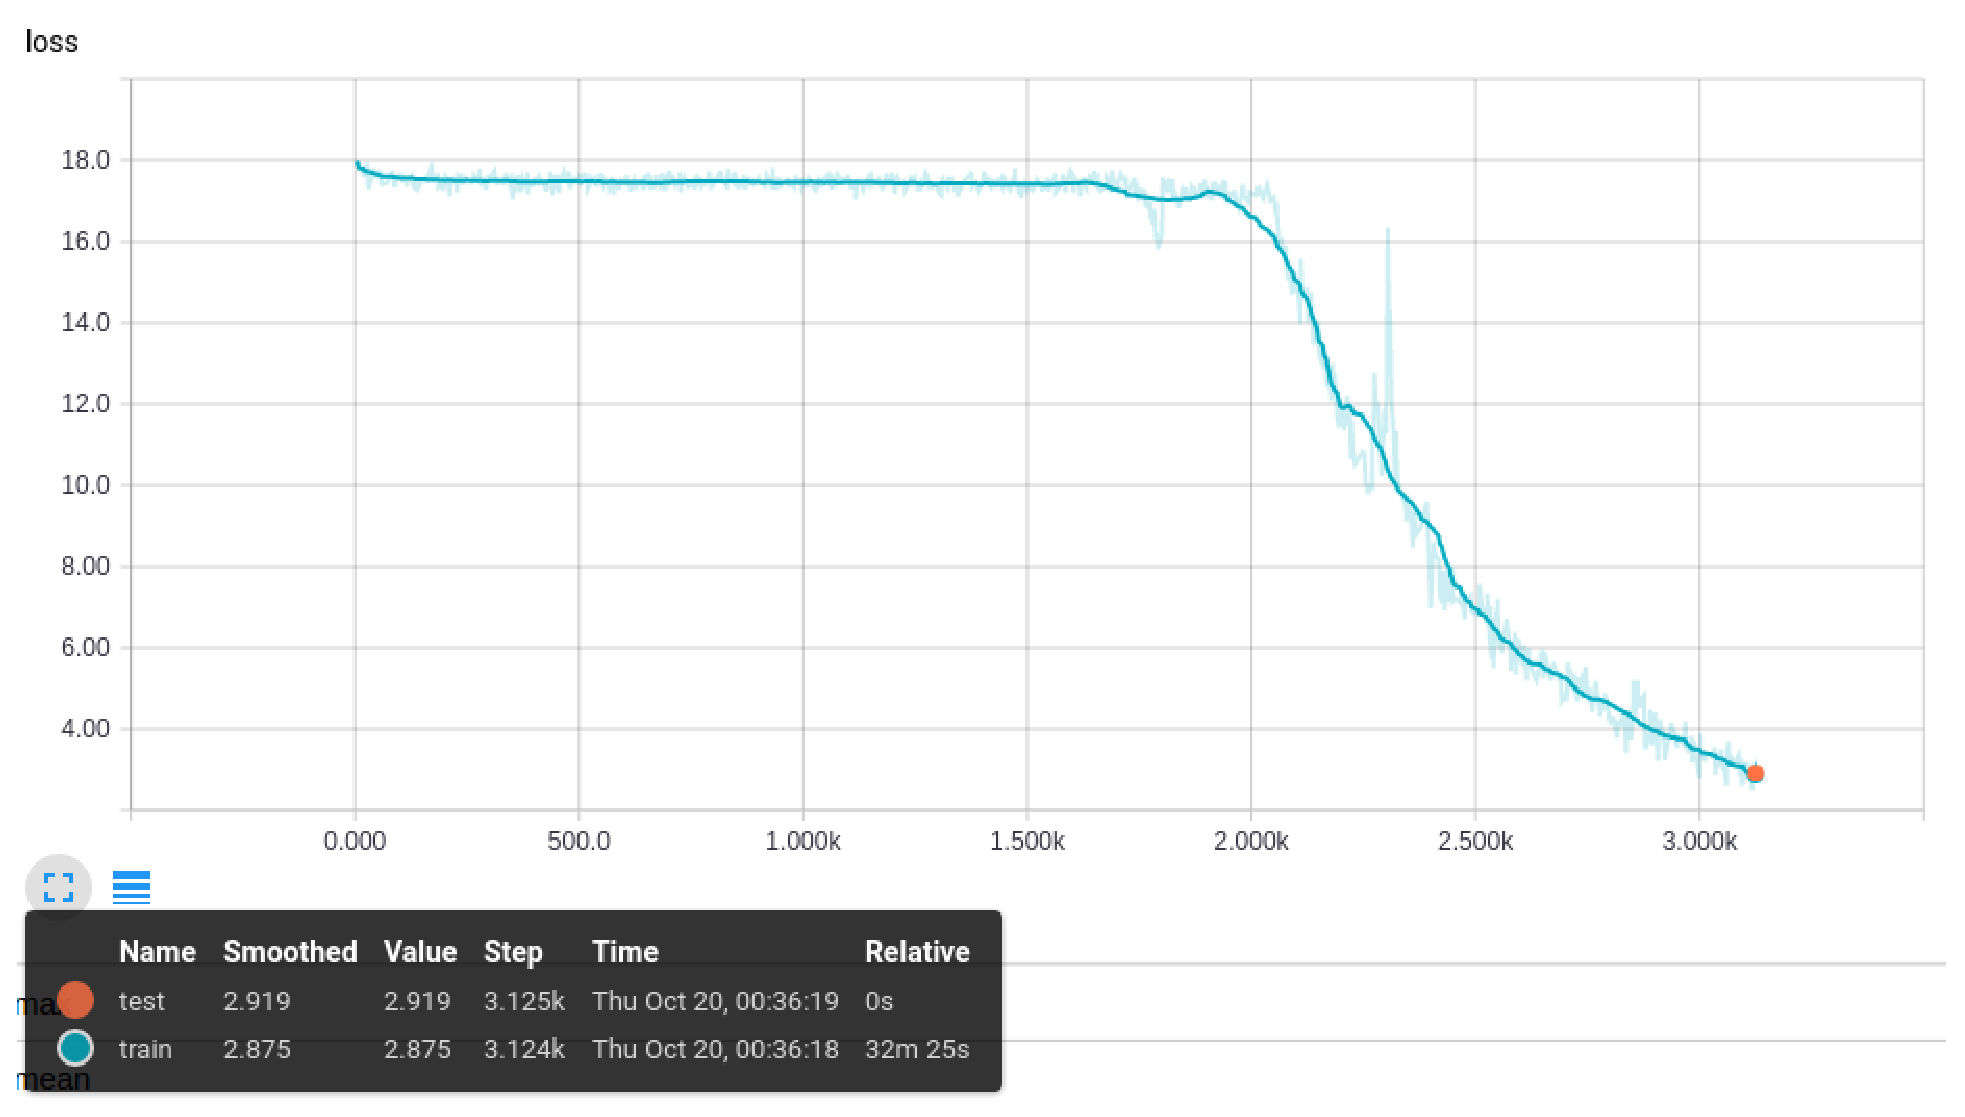
\includegraphics[scale=0.4]{imagens/loss_200k}
\caption{Gráfico da perda em relação ao número de passos para o
  treinamento da rede com 200 mil iterações.}
\label{fig:loss_200k}
\end{figure}

Mesmo com o bom resultado nos testes, foi notado uma falta de
estabilidade nos gráficos gerados. Analisando os gráficos de desvio
padrão dos valores de pesos e \textit{biases} das últimas camadas
convolucionais, percebe-se que alguns valores poderiam continuar
alterando se o treinamento continuasse por mais iterações.

\begin{figure}[H]
\centering
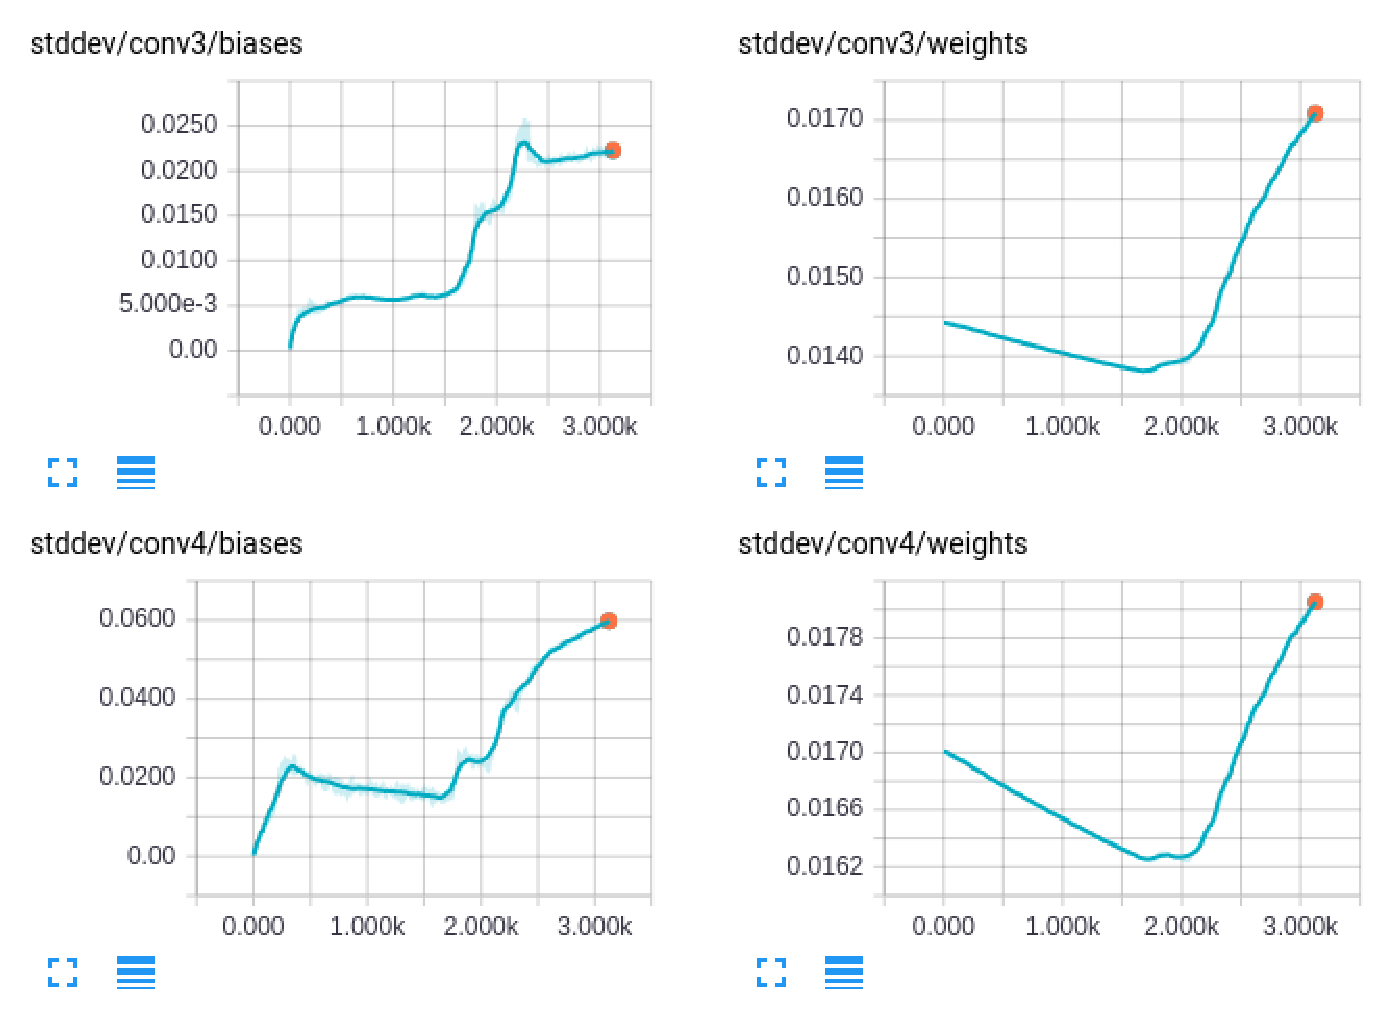
\includegraphics[scale=0.6]{imagens/stddev_200k}
\caption{Desvio padrão dos pesos e \textit{biases} em relação ao
  número de passos para o treinamento da rede com 200 mil iterações.}
\label{fig:stddev_200k}
\end{figure}

\section{Treinamento com 500 mil iterações}

Visto a instabilidade nos valores de gráficos no treinamento anterior,
a tentativa seguinte foi aumentar o número de iterações para 500 mil,
portanto 7.812 passos. O tempo total de treinamento foi de {\bf 1 hora
18 minutos e 23 segundos}.

Analisando os gráficos gerados com este treinamento, novamente o valor
da perda para oscila entre 16,87 e 17,51 até um certo ponto. Dessa vez
é no passo número 2.922 (iteração 187.008) onde a perda começa a
decair. O mesmo acontece com a acurácia, ficando em torno de 6\% até o
passo 2.977 (iteração 190.528) quando começa a subir. Ao final do
treinamento foi alcançada uma acurácia de {\bf 97,81\%} no conjunto de
treinamento, {\bf 81,37\%} no conjunto de teste e uma perda de {\bf
  0,43} para o conjunto de treinamento, {\bf 13,52} para o conjunto de
teste.

\begin{figure}[H]
\centering
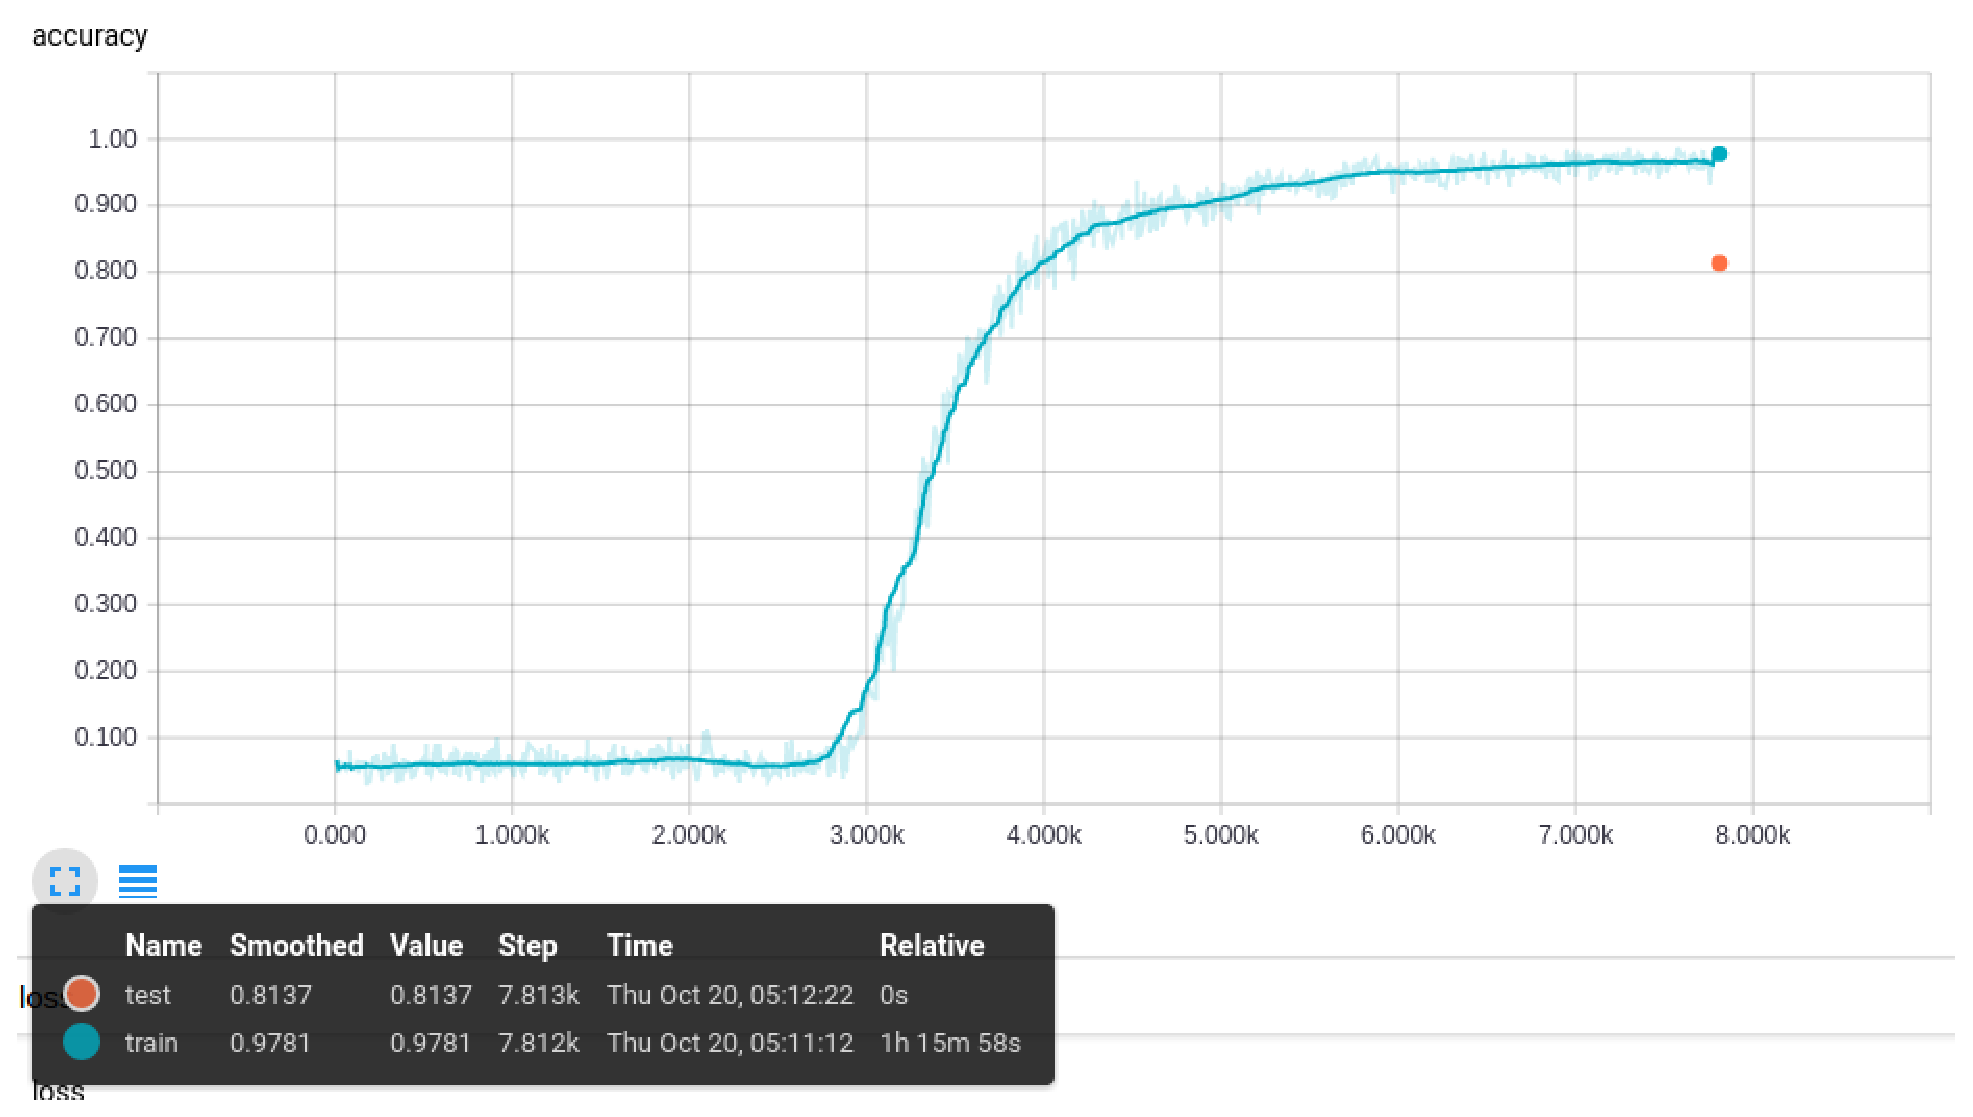
\includegraphics[scale=0.4]{imagens/accuracy_500k}
\caption{Gráfico da acurácia em relação ao número de passos para o
  treinamento da rede com 500 mil iterações.}
\label{fig:accuracy_500k}
\end{figure}

\begin{figure}[H]
\centering
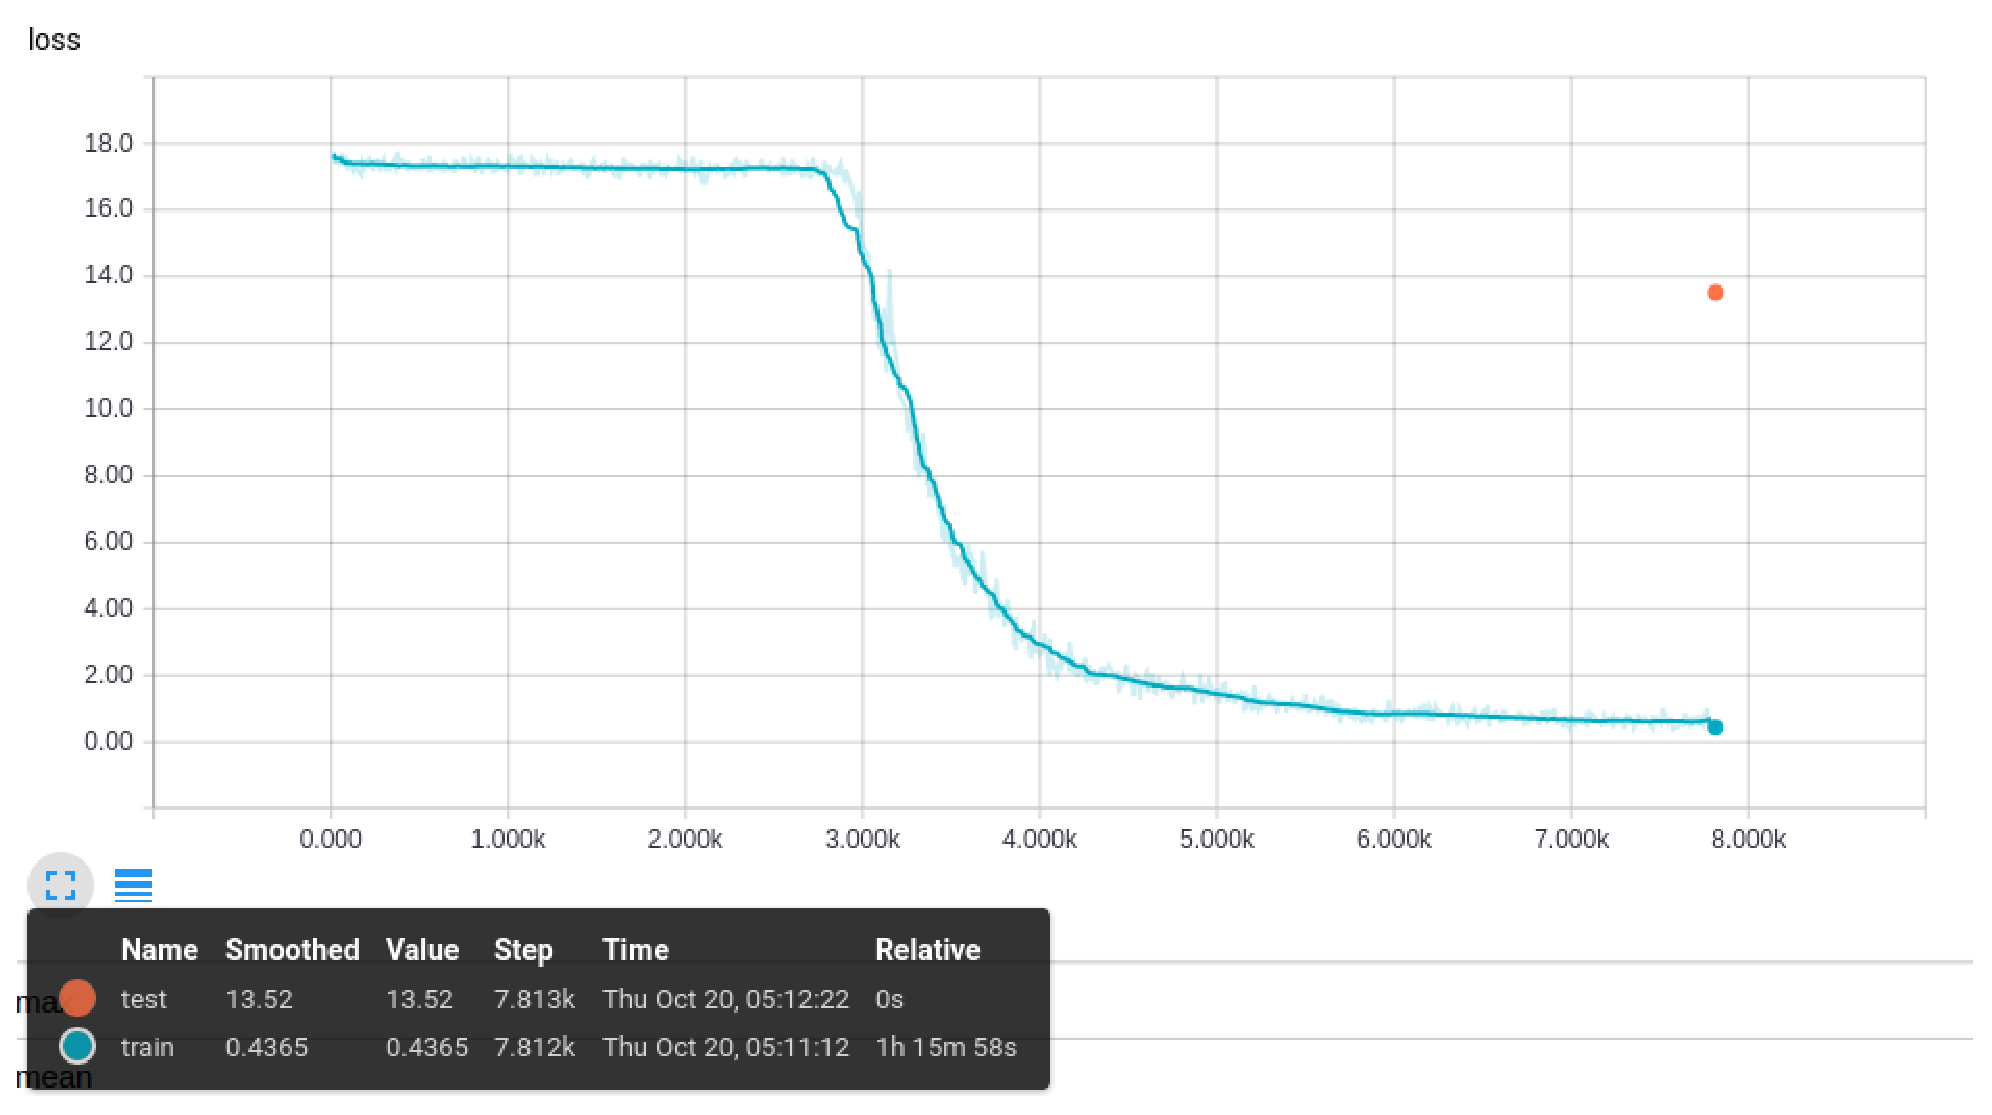
\includegraphics[scale=0.4]{imagens/loss_500k}
\caption{Gráfico da perda em relação ao número de passos para o
  treinamento da rede com 500 mil iterações.}
\label{fig:loss_500k}
\end{figure}

Analisando os resultados, é possível observar que o valor da perda
para o conjunto de treinamento é muito diferente do valor da perda
para o conjunto de teste. Também nota-se que a acurácia no conjunto de
treinamento chegou bem perto de 100\%. De acordo com a fundamentação
teórica, esses dois fatores podem ter sido causados pelo
\textit{overfitting} do modelo ao conjunto de dados do treinamento.

\section{Treinamento com 500 mil iterações e Dropout de 50\%}

Na tentativa de minimizar os problemas encontrados anteriormente, foi
realizado um terceiro treinamento. Foi visto que uma das técnicas de
regularização para minimizar o \textit{overfitting} é adicionando uma
camada de \textit{dropout} ao modelo. Nossa arquitetura já previa uma
camada de \textit{dropout}, no entanto o parâmetro de probabilidade de
mantimento das ativações estava configurado para 75\% (0,75). Para o
terceiro treinamento foi configurada a probabilidade do
\textit{dropout} para 50\% (0,5) e assim analisados os resultados. O
tempo total de treinamento foi de {\bf 1 hora 18 minutos e 53
  segundos}.


\begin{figure}[H]
\centering
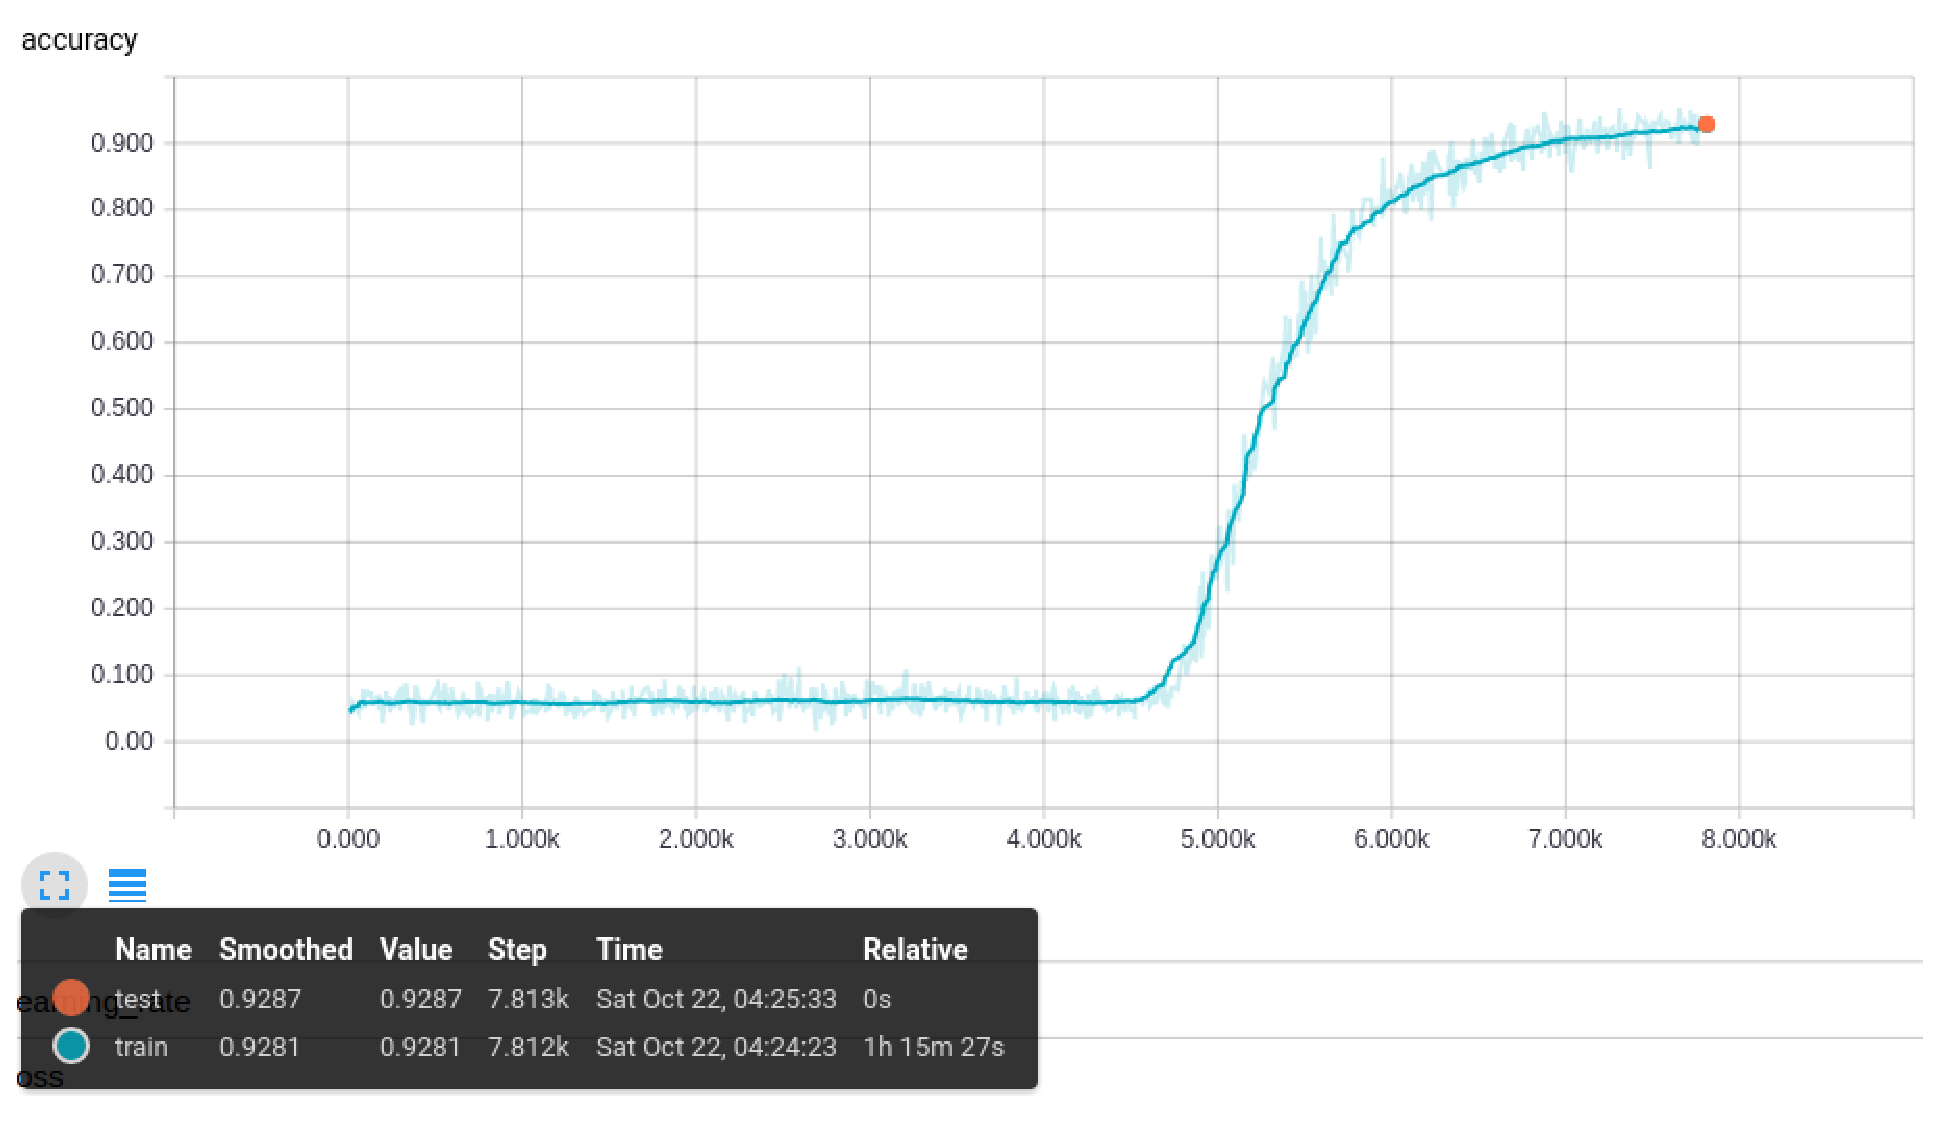
\includegraphics[scale=0.4]{imagens/accuracy_500k_dropout50}
\caption{Gráfico da acurácia em relação ao número de passos para o
  treinamento da rede com 500 mil iterações e probabilidade de
  \textit{dropout} igual a 50\%.}
\label{fig:accuracy_500k_dropout50}
\end{figure}

\begin{figure}[H]
\centering
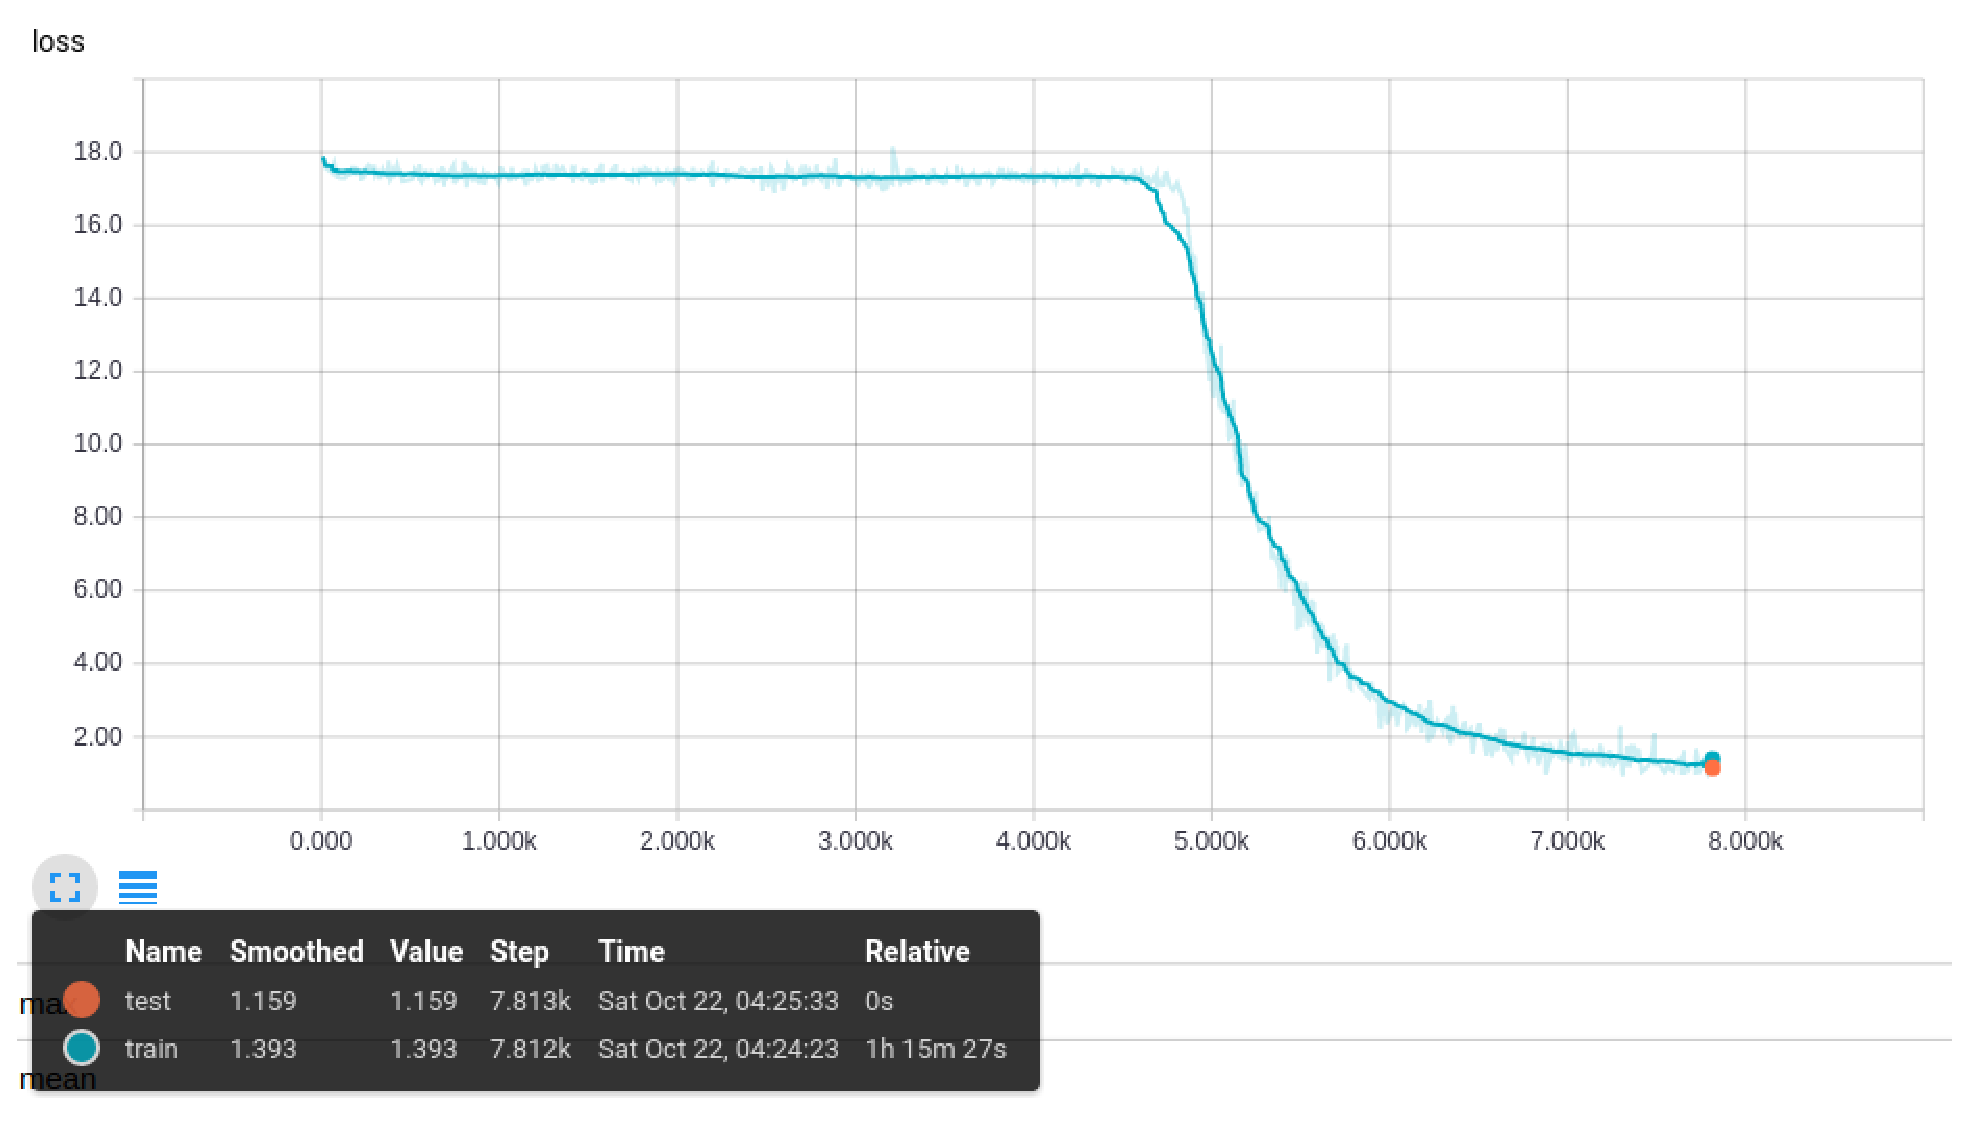
\includegraphics[scale=0.4]{imagens/loss_500k_dropout50}
\caption{Gráfico da perda em relação ao número de passos para o
  treinamento da rede com 500 mil iterações e probabilidade de
  \textit{dropout} igual a 50\%.}
\label{fig:loss_500k_dropout50}
\end{figure}

Ao final do treinamento foi alcançada uma acurácia de {\bf 92,81\%} no
conjunto de treinamento, {\bf 92,87\%} no conjunto de teste e uma
perda de {\bf 1,39} para o conjunto de treinamento, {\bf 1,15} para o
conjunto de teste. Vale lembrar que durante a fase de treinamento o
algoritmo de otimização passa por uma carga de imagens completamente
diferente em cada passo executado. Já na fase de teste o algoritmo
passa por todas as 8 mil imagens de teste de uma só vez e fornece os
valores registrados. Portanto no conjunto de treinamento os gráficos
mostram que a acurácia chegou a {\bf 95,31\%} e a perda chegou a {\bf
  0,93} mas os valores registrados para estudo são os últimos valores de
saída do treinamento.

\section{Resultados}

De acordo com os testes realizados a configuração de alguns parâmetros
no treinamento foram essenciais para eficácia do sistema proposto.

\begin{table}[H]
\begin{center}
\begin{tabular}{|p{2.3cm}|p{2.3cm}|p{2.3cm}|p{2.3cm}|p{2.3cm}|}
\hline
\textbf{} & \textbf{200k it.} & \textbf{500k it.} & \textbf{500k it. e 50\% \textit{dropout}} \\
\hline
Acurácia (teste) & {\bf 79,6\%} & {\bf 81,37\%} & {\bf 92,87\%} \\
\hline
Acurácia (treinamento) & 80,94\% & 97,81\% & 92,81\% \\
\hline
Perda (treinamento) & 2,87 & 0,43 & 1,39 \\
\hline
Perda teste & 2,91 & 13,52 & 1,15 \\
\hline
\end{tabular}
\caption{Desempenho geral do sistema.}
\label{tab:system_efficency}
\end{center}
\end{table}
